% Acertar titulo do capitulo

A internet apresenta um crescimento exponencial no mundo atual.
Estima-se que no ano de 2016 cerca de 66\% da população brasileira tenha acesso à rede \cite{social17}.
Ela é usada massivamente no dia a dia das pessoas, estando presente desde a realização de tarefas básicas e essenciais,
como cozinhar e se locomover numa cidade, até o preenchimento do tempo de lazer, com vídeos, notícias, mensagens
instantâneas e redes sociais.
% Falar sobre o uso da internet, ubuiquidade e etc

Através especialmente das redes sociais, a internet modificou a forma de interação entre as pessoas.
No Brasil, 58\% da população, ou seja, 120 milhões de pessoas, participam de pelo menos uma rede social, gastando em
média, 220 minutos por dia no ano de 2016~\cite{social17}.
Isso faz do Brasil o segundo país em tempo navegando em redes sociais, atrás apenas das Filipinas~\cite{social17}.
Isso não só cria uma nova instância de comunicação entre as pessoas, mas também abre um lugar para a expressão dos
sentimentos e opiniões de cada um.
Com isso, após o surgimento das redes sociais, a presença online deixou de ser uma comunicação de via única.
Agora, os leitores interagem com a fonte de informação recebida, seja ela uma notícia, atualização de amigos, etc.

Essa presença central das mídias sociais na vida das pessoas faz com que os usuários passem a ser mais influenciados
por opiniões que trafegam pela mesma.
Desta maneira, as redes sociais passam a ter um peso maior na tomada de decisão de cada individuo, como na compra de
um produto ou na escolha de um candidato para a ser votado.
O impacto destes novos meios de comunicação podem ser observados, por exemplo, nas mobilizações de massa ocorridas na
primavera árabe em 2011 que levaram a queda de governos no qual as mídias sociais exerceram papel
crítico~\cite{mourtada11}.

Nesse sentido, tornaram-se necessários trabalhos que analisem o que se está dizendo nas redes sociais.
Para uma emissora de TV, por exemplo, é interessante saber o que está sendo dito sobre sua programação, assim como para
a assessoria de um cantor, é importante descobrir se sua nova canção está agradando ou não seu público.

Jim Yu, presidente da empresa de marketing digital BrightEdge, ressalta que os sentimentos expressos por clientes em
relação a uma marca é uma das principais métricas de \textit{branding}~\cite{marketingland}.
O colunista da Forbes, Daniel Newman, destaca que a utilização de técnicas de análise de sentimento em conjunto com
outras técnicas de \textit{big data} vem revolucionando a forma de se fazer marketing, permitindo uma maior
personalização dos produtos e fortalecimento de relação com os clientes~\cite{newman16}.

Entretanto, a criação de conteúdo digital acompanha o crescimento da internet.
No ano de 2016, a cada sessenta segundos foram adicionadas 500 horas vídeo no YouTube, realizadas 3.8 milhões de buscas
no Google e publicados 450 mil \textit{tweets}~\cite{smartinsights}.
Estes números tornam impraticável a realização de análise de sentimento manualmente sobre mídias com esse volume de
dados.
Portanto, a utilização de métodos de automatizados é um modo de viabilizar a realização dessa tarefa.
Porém, a extração de informação de linguagem natural não é uma tarefa simples, pois envolve conhecimentos da língua
explícitos e implícitos, regulares e irregulares, sintáticos e semânticos~\cite{cambria13}.
Sobretudo, a análise de sentimento ainda envolve problemas ainda não resolvidos no processamento de linguagem
natural~\cite{cambria13}
como a resolução de correferências~\cite{soon01}, resolução de anáforas~\cite{lappin94}, reconhecimento de
entidades~\cite{nadeau07} e ambiguidade de palavras~\cite{yarowsky95}.
Estes fatores constituem desafios adicionais para a tarefa.

\section{Análise de Sentimento}

O campo de estudos da análise de sentimento, também chamado de mineração de opinião, é um dos ramos mais ativos do
processamento de linguagem natural~\cite{liu12}.
A análise de sentimento tem como objetivo analisar a opinião, a avaliação, a emoção e a atitude de um documento em
relação a um evento, produto, serviço, organização, ou qualquer outra entidade.
Apesar do processamento de linguagem natural ter um longo histórico de estudos, a análise de sentimento se consolidou
apenas no inicio dos anos 2000 com a crescente demanda comercial.
Observa-se que o crescimento de interesse nessa área tem grande correlação com o crescimento de mídias sociais e do
volume de dados, visto que o sucesso das redes sociais disponibilizam quantidades massivas de dados possibilitando tanto
a oferta de novas aplicações quanto oportunidades de desenvolvimento de técnicas~\cite{liu12}.

O campo de análise de sentimento apresenta diferentes subáreas de estudo.
Dentre elas, a tarefa mais presente na literatura e que abordaremos neste trabalho é a análise de polaridade de um
documento.
A análise de polaridade visa classificar textos em uma escala entre positivo e negativo.
Encontra-se também estudos que visam determinar a subjetividade ou objetividade de um texto, como no trabalho de Wiebe e
Rilof~\cite{Wiebe05}.
Também entra no escopo de análise de sentimento a classificação de emoções presentes em uma mensagem, como felicidade,
raiva, tristeza, etc~\cite{bollen11b}.
Outro foco de pesquisa com grande aplicações práticas é a análise de sentimento porém, não da mensagem como um todo, mas
do sentimento em relação a uma entidade presente na mensagem~\cite{eirinaki12}.
O contrário também é possível, a análise da influência do sentimento de um termo em relação a mensagem~\cite{socher13}.
Percebe-se que a análise de sentimento se desmembra em varias subdivisões e novas subdivisões surgem a cada dia visto
que a área ainda está em processo de expansão, o que confirma seu grande potencial de aplicação.

Com o crescimento da participação dos usuários na formação de conteúdo da Web torna-se cada vez mais relevante a análise
do conteúdo sendo produzido.
Zhuang \textit{et al.}~\cite{zhuang06}, por exemplo, utiliza mineração de opinião para extrair avaliações a partir de
críticas de filmes feitas por usuários.
Hu e Liu~\cite{hu04}, por sua vez, desenvolveram métodos para resumo de sentimento de avaliações de produtos vendidos
por comercio eletrônico.

A utilização de classificadores de opinião sobre dados de redes sociais se mostrou relevante em diversas aplicações.
Bollen \textit{et al.}~\cite{bollen11}, por exemplo, aplicam análise de sentimento de mídias sociais para predição de
mercados financeiros.
Tumasjan \textit{et al.}~\cite{tumasjan10}, por sua vez, utilizam o sentimento exposto no Twitter para prever resultados
eleitorais.
Até mesmo na predição de bilheteria de filmes, como feito por Du \textit{et al.}~\cite{du14}.

Porém, a produção de base de dados para o treinamento de modelos de aprendizado supervisionado é um processo custoso.
O seu processo de desenvolvimento envolve a anotação manual de dados, preferencialmente por múltiplas pessoas.
Contudo, apesar de modelos simples como os obtidos com técnicas como Naïve Bayes e \textit{Support Vector Machines}
conseguirem desempenhos satisfatórios com quantidades limitadas de dados, modelos mais complexos como redes neurais
profundas dependem de grandes volumes de dados para obter êxito, tornando o processo de anotação manual extremamente
ineficiente.
Sobretudo, uma vez formada esta base de dados, ela só é eficiente para o desenvolvimento de classificadores aplicados
na mesma língua, no mesmo formato, e sem grandes defasagens de tempo.
Por exemplo, uma base de dados composta por \textit{tweets} seria ineficiente para modelagem de classificadores de
emails, ou mesmo o uso de uma base formada por \textit{tweets} de 2010 sofreria queda de performance se o modelo
treinado com esta for aplicado em \textit{tweets} de 2018, visto a evolução da língua neste período de tempo.

Portanto, se faz necessário desenvolver métodos como o apresentado por Go \textit{et at.}~\cite{go09}, que desenvolve
uma base composta de \textit{tweets} a partir de anotação automática por \textit{emoticons}.
O trabalho de Go \textit{et at.}~\cite{go09} visa definir um sistema de classificação de sentimento sem a necessidade de
anotação manual dos dados para treinamento, utilizando supervisão distante, técnica de anotação ruidosa automática.
Neste artigo a análise de sentimento tratada é a extração de polaridade, negativa ou positiva, de uma mensagem.
Em especial, as mensagens desse trabalho são originárias do Twitter, serviço de microblogs, sendo este trabalho o
primeiro a estudar este tipo de mensagem.

% colocar exemplos compativeis com os apresentados anteriormente
Por ser uma plataforma aberta, o Twitter é composto de mensagens dos mais diversos domínios.
Esse fator dificulta a tarefa de classificação a ser executada quando comparado com trabalhos de um domínio específico,
como por exemplo a análise de sentimento para avaliação de filmes a partir de resenhas; ou na predição de flutuações do
mercado financeiro pela análise de artigos jornalísticos.

A Tabela~\ref{tab:sentiment} exemplifica a classificação de polaridade de \textit{tweets}, foco deste trabalho.
As mensagens presentes nessa tabela são transcrições de \textit{tweets} reais selecionados de maneira a ilustrar
a classificação de sentimento.

\begin{table}[h]
    \begin{center}
        \begin{tabular}{| l | p{10cm} |}
        \hline
        \textbf{Sentimento} & \textbf{\textit{Tweet}} \\ \hline
        Positivo & Grande notícia, João Sousa e Gastão Elias representam Portugal nos Jogos Olímpicos do Rio de Janeiro.
        \\ \hline
        Neutro & Entrevistei hoje a Priscilla Carnaval do BMX. Classificada para o \#Rio2016, ela tem novidades na
        preparação olímpica. \\ \hline
        Negativo & Estão transformando Olimpíadas que é algo sério num espetáculo triste e de mau gosto. \\ \hline
        \end{tabular}
        \caption{Exemplo de classificação de sentimento em \textit{tweets}.}
        \label{tab:sentiment}
    \end{center}
\end{table}

Entretanto, nem todos exemplos são claramente distinguíveis como os apresentados na Tabela~\ref{tab:sentiment}.
A comunicação frequentemente apresenta fatores como ironia, ambiguidade de sentimentos e multiplicidade de idiomas.
Em outros casos, a mensagem sendo analisada pode ser complementar a mensagens anteriores ou informações não textuais
que a acompanham.
Estes fatores são complexidades adicionais e diminuem a acertividade dos classificadores.
A Tabela~\ref{tab:sentiment_complexity} demonstra exemplos das dificuldades indicadas.

\begin{table}[h]
    \begin{center}
        \begin{tabular}{| l | p{10cm} |}
        \hline
        \textbf{Fator} & \textbf{\textit{Tweet}} \\ \hline
        Ironia & Recomendo chegar para dar aula e descobrir que mudaram seu horário sem avisar. \\ \hline
        Ambiguidade & Estou igualmente fascinada e enojada. \\ \hline
        Multiplicidade de idiomas & Macarrão de arroz is the new miojo. \\ \hline
        \end{tabular}
        \caption{Dificuldades encontradas na classificação de sentimento.}
        \label{tab:sentiment_complexity}
    \end{center}
\end{table}

\section{Twitter}

O Twitter é um microblog e rede social no qual os usuários interagem a partir de mensagens, chamadas \textit{tweets}.
Microblogs são meios de comunicação que permitem usuários a compartilhar conteúdos e mídias.
As principais características dos microblogs são a brevidade e instantaneidade.
Os \textit{tweets} são limitados a 140 caracteres e podem conter fotos, vídeos, links, localizações referências a
usuários e \textit{hashtags}.
Criada em 2006, a rede social cresceu rapidamente a ponto de se tornar uma das redes com maior número de usuários no
mundo.
No ano de 2016 o Twitter a plataforma contava com a presença de 330 milhões de usuários ativos por mês.
A Figura~\ref{fig:tweet_ex} mostra um exemplo de \textit{tweet}.

\begin{figure}
\begin{center} {
    \begin{center}
    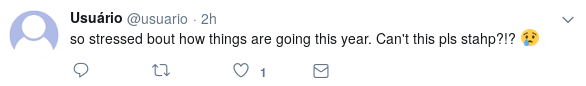
\includegraphics[scale=0.7]{tweet-example.png}
    \caption{Exemplo de \textit{tweet} contendo \textit{emoticon}, abreviação e neologismos.}
    \small{As informações do usuário foram anonimizadas para sua privacidade.}
    \label{fig:tweet_ex}
    \end{center}
}
\end{center}
\end{figure}

Um ponto chave da comunicação por Twitter são as \textit{hashtags}.
\textit{Hashtags} são palavras-chave ou frases que definem um tópico ou tema.
Elas são caracterizadas por serem precedidas pelo simbolo da tralha (\#) e por não conterem espaços ou pontuação.
São, ainda, elementos clicáveis que apontam o leitor para outra página.
Essa outra página, por sua vez, contém um mural com todas as citações contendo aquela \textit{hashtag}.
Desta forma, \textit{hashtags} funcionam como agregadores de \textit{tweets}.

O tamanho reduzido das mensagens veiculadas por Twitter e o meio pelo qual elas circulam levam a utilização de
variações gramaticais da língua especificas para este ambiente.
É comum encontrar, por exemplo, o uso excessivo de abreviações para reduzir a contagem total de caracteres, a repetição
de pontuação para reforçar intensidade e o uso de neologismos.

Se tratando de classificação de sentimento, o fato do tamanho reduzido e linguagem própria apresentam uma dificuldade
adicional.
Apesar de não serem abordadas nesse trabalho, atributos não textuais como: republicação ou citação de mensagem, presença
de foto ou vídeo, grafos de conexões entre usuários etc podem colaborar na realização da tarefa de análise de sentimento.
